% A simple template for LaTeX documents
% 
% To produce pdf run:
%   $ pdflatex paper.tex 
%


\documentclass[12pt]{article}

% Begin paragraphs with new line
\usepackage{parskip}  

% Change margin size
\usepackage[margin=1in]{geometry}   

% Graphics Example:  (PDF's make for good plots)
\usepackage{graphicx}               
% \centerline{\includegraphics{figure.pdf}}

% subfigures, side by side
\usepackage{subcaption}

% hyperlinks
\usepackage{hyperref}

% Blocks of code
\usepackage{listings}
\lstset{basicstyle=\ttfamily, title=\lstname}
% Insert code like this. replace `plot.R` with file name.
% \lstinputlisting{plot.R}

% Monospaced fonts
%\usepackage{inconsolata}
% GNU \texttt{make} is a nice tool.

% Supports proof environment
\usepackage{amsthm}

% Allows writing \implies and align*
\usepackage{amsmath}

% Allows mathbb{R}
\usepackage{amsfonts}

% Numbers in scientific notation
% \usepackage{siunitx}

% Use tables generated by pandas
\usepackage{booktabs}

% Allows umlaut and non ascii characters
\usepackage[utf8]{inputenc}

% norm and infinity norm
\newcommand{\norm}[1]{\left\lVert#1\right\rVert}
\newcommand{\inorm}[1]{\left\lVert#1\right\rVert_\infty}

% Statistics essentials
\newcommand{\iid}{\text{ iid }}
\newcommand{\Exp}{\operatorname{E}}
\newcommand{\Var}{\operatorname{Var}}
\newcommand{\Cov}{\operatorname{Cov}}


%%%%%%%%%%%%%%%%%%%%%%%%%%%%%%%%%%%%%%%%%%%%%%%%%%%%%%%%%%%%

\begin{document}

\title{Parallel Computing Through Code Analysis}
\date{\today}
\author{Clark Fitzgerald}
\maketitle

\begin{abstract}

    Users begin by writing correct R code.  We then analyze their code, and
    transform it into a version which is tailored to the data and the
    capabilities of the platform. This could mean splitting data into
    appropriately sized chunks and using multiprocessing. More ambitiously,
    it could mean transferring data and compiling code for a GPU (graphical
    processing unit).

\end{abstract}

This is a prospectus for distribution to the committee for PhD
Qualifying Exam in June 2017.

For principled, optimal approaches to parallel chunked computations we
first have to understand their performance characteristics.

One could think about this as a system architecturally organized in layers- building on
partools, say, which builds on SNOW. Users are free to enter at any layer.

Idea for metadata- see notes in partools. Could use a data structure
describing characteristics for how each chunk of the data is accessed,
ideally along with something about the sizes.

\section{An Example}
%%%%%%%%%%%%%%%%%%%%%%%%%%%%%%%%%%%%%%%%%%%%%%%%%%%%%%%%%%%%

The California Department of Transportation collects traffic
data through sensors embedded in highways. These detectors count passing
vehicles, measure activation time, and estimate their average velocity \cite{jia2001pems}.
Every thirty seconds they produce a new data point. $43,680$ sensors in
California $\times 3$ parameters $\times (2 \times 60 \times 24)$
measurements per day results in 377 million new data points per day.
This raw data is organized into files by management district and day and is
publicly available to download.

As an analyst I would like to perform a statistical computation involving a
robust regression for each sensor. From the R language this can be done
easily and efficiently, for example with the \texttt{rlm} (robust linear
model) function in the MASS package \cite{venables2013modern}.

However, the size and organization of the data makes the task much more
difficult.  I've downloaded a subset of the data consisting of measurements
in the San Francisco Bay Area for part of 2016. This takes up hundreds of
gigabytes, so it will not fit in memory.

It would be easier to perform the regression if the data were
organized in files for each sensor rather than in files for each day.  One
approach then is to reorganize the data on disk into this file structure. I
did this using a simple single threaded R program, and it took 23 hours to
run on 134 GB of data.

This is a poor level of performance.  Another drawback is that it
requires specific custom code. Parallelizing and tuning it makes it even
more specific to the data and platform.

What if I didn't have to write this custom code? What if we had a system
that could inspect the idiomatic R code that one would write to perform an
operation as if the data were small, and then automatically take steps to
scale and to parallelize the operations? It could also tune them for the
specifics of the system and the data. This is what I'm working towards.

\subsection{Code, Data, Platform}
%%%%%%%%%%%%%%%%%%%%%%%%%%%%%%%%%%%%%%%%%%%%%%%%%%%%%%%%%%%%

Duncan Temple Lang deserves credit for the following idea:
\textbf{Code} is the R (or whatever language) script to be executed.
\textbf{Data} could be single or multiple files, a database, a parallel
file system, etc.  \textbf{Platform} is the physical hardware, such as a
CPU with 8 cores or 2 GPUs with a high end connection. The combination of
(Code, Data, Platform) dictates what strategies should be used for
efficient evaluation.

If the data is ``small enough'' then performance will be acceptable no
matter regardless of how well the platform is utilized and how efficient
the code is. Conversely, if the data is ``large enough'' then
\emph{everything} matters, since small inefficiencies will be magnified
when they occur millions of times.

\subsection{Data Movement}
%%%%%%%%%%%%%%%%%%%%%%%%%%%%%%%%%%%%%%%%%%%%%%%%%%%%%%%%%%%%

Moving data is slow and therefore should be minimized. It can be slow in
terms of latency and also because of bandwidth. Examples of this include
transferring data over a network, where latency can be measured in
milliseconds and bandwidth in MB per second.

Initially assume that the code is correct. Consider an example of code that
reads a file, performs a computation, and saves the result in a file.
Most approaches to improving performance or scaling to large datasets
come from \emph{manually rewriting} the code, tailoring it to this
particular application. It's better to avoid this if possible.  Code that's
rewritten for performance results in an increase in complexity
\cite{matloff2015parallel}.  Compilation is one way to keep the original
code and get more speed. Translation and metaprogramming are another way.
Translation here refers to taking the code and modifying it, for example by
adding statements.


\section{Approximating data size}
%%%%%%%%%%%%%%%%%%%%%%%%%%%%%%%%%%%%%%%%%%%%%%%%%%%%%%%%%%%%

For data in files one could read the first several records along with the
data size and make an inference as to how many rows there are, and come up
with an appropriate evaluation scheme. This is similar to how column
inferences work.

\section{Introduction}
%%%%%%%%%%%%%%%%%%%%%%%%%%%%%%%%%%%%%%%%%%%%%%%%%%%%%%%%%%%%

What new things am I bringing to the table? My QE is in two months, time to
focus.

General idea- code analysis to detect and use parallelism. Determining and
using a chunking scheme based on (code, platform, data).

Running without chunks is the same as regular vectorized R- one can think
of this as a degenerate case of chunked operations with just one chunk.

Broad idea- more separation between the high level language
and the implementation. This is consistent with the idea of R as a `wrapper'
language, providing a convenient interface for numerical routines written
in a faster language \cite{chambers2016extending}.

Right now seems like a very good time to be pursuing this, since many of the
building blocks are in place:
\begin{itemize}
    \item Fast IO packages
    \item SNOW and parallel
\end{itemize}

partools in particular is a nice base to build on.

Code analysis seems like the most esoteric thing compared to the others.

Some functions can be applied in a streaming manner, where they visit the
data. Can we detect these functions programmatically? If we can then this
gives free parallelism.

I'd like to examine the code and determine where parallelism will give the
most benefit. Ie. nesting parallelism will likely hurt. But how much? And
can we detect it?

\section{Small Data and Overhead}
%%%%%%%%%%%%%%%%%%%%%%%%%%%%%%%%%%%%%%%%%%%%%%%%%%%%%%%%%%%%




\section{Big Data and Swapping}
%%%%%%%%%%%%%%%%%%%%%%%%%%%%%%%%%%%%%%%%%%%%%%%%%%%%%%%%%%%%

What happens when data is too big? One runs into algorithmic limitations as
well, ie. $O(n^2)$ operations become very expensive for large $n$.

R can do some computations out of memory through the use of the system
swap. Swap space aka ``virtual memory'' is a portion of the hard drive that
the host operating system allocates for memory to spill over into so that
the computer doesn't run out of memory.  Exceeding the physical memory on
the system causes several problems.

First, data that's too big will still fail. Swap space is typically
around the same size as memory. For example, my Ubuntu Linux desktop has
8GB of RAM and 8GB of swap space on a spinning disk (not an SSD). Objects
in R can't take up more space than the size of memory plus the size of
swap. Here's a typical error:

\begin{verbatim}
> trillion = 1e12
> x = rnorm(trillion)
Error: cannot allocate vector of size 7450.6 Gb
\end{verbatim}

Second, computation is much faster if the data fits in memory.
Figure \ref{fig:spinning_disk_swap} shows what happens to run time when
simply computing the mean of $n$ random numbers, for $n$ chosen to create a
vector pushing the limits of memory.\footnote{Note that this computation
could just as easily be done in a streaming fashion, producing random
numbers, updating the mean, and then discarding them.} For vectors using between $(0.1, 0.85)$
of the available memory the timings are linear as expected.
Once the computation spills into swap space the timings immediately become
worse by an order of magnitude, and they are less predictable.

Lastly, loading data from disk into memory and then swapping back into disk
is fundamentally inefficient. The data was already read from disk once, why force it
to be read again in this way if we can avoid it?

\begin{figure}
\centering
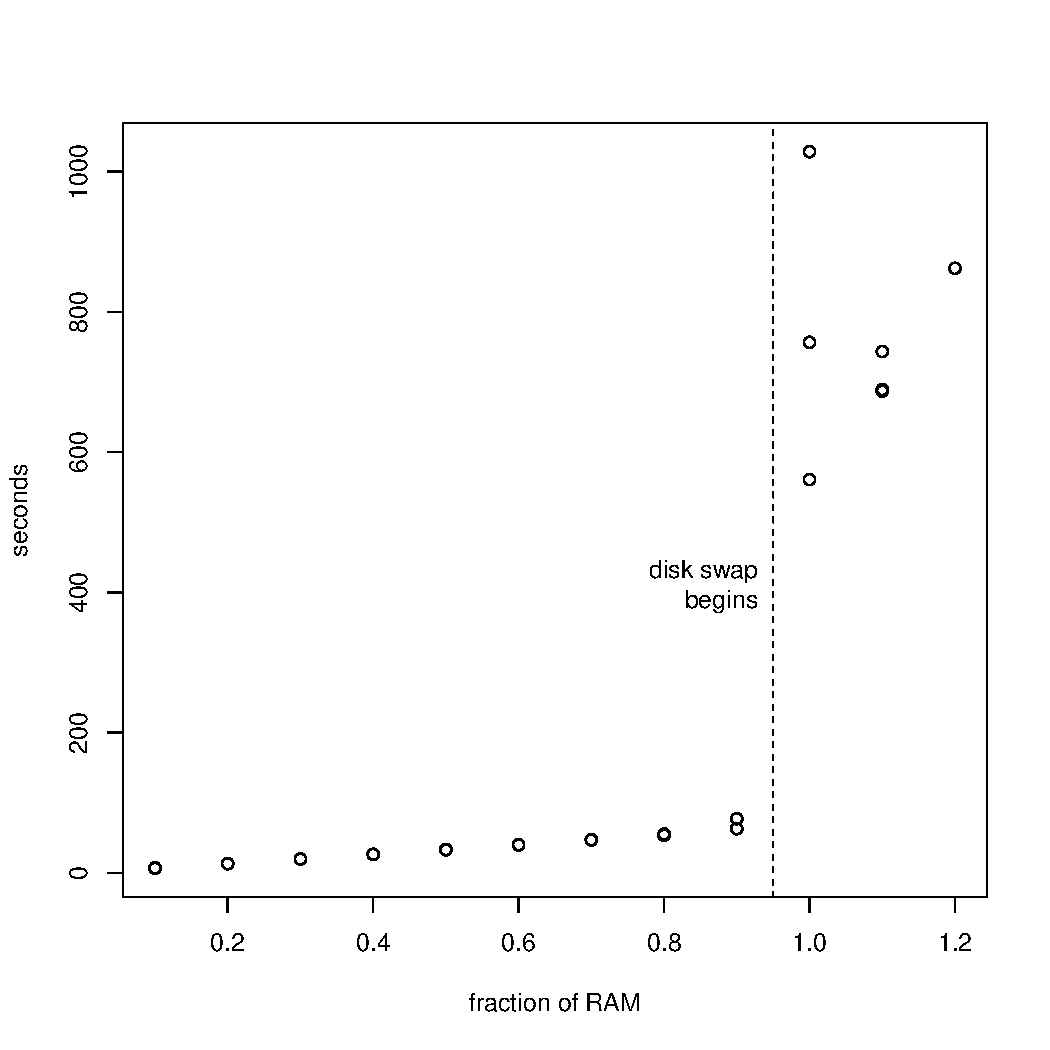
\includegraphics[width=.8\linewidth]{swap/spinning_disk_swap}
\caption{Performance is reasonable while data fits in memory.}
\label{fig:spinning_disk_swap}
\end{figure}

Compilation can alleviate this issue, but it can't resolve it, since it
can't give the system more memory. It may be able to help reduce the
creation of large intermediate data objects.


\section{Chunking Approaches to Large Data}
%%%%%%%%%%%%%%%%%%%%%%%%%%%%%%%%%%%%%%%%%%%%%%%%%%%%%%%%%%%%

To stay in memory we use chunked computations. If the chunks are too small
they'll be inefficient. Then how do we choose the chunk size?  There may be
a ``sweet spot'' or range of values for computation as well as for
statistical accuracy. For example, for software alchemy to work it's
necessary that the chunk sizes increase towards infinity
\cite{matloff2014software}.



\textbf{Speculative evaluation of different chunked computation schemes}

A well known technique for parallel computation is to split data into
chunks and compute on each chunk simultaneously. This approach 
is useful on large data. Multiplying large block matrices is an example of this.

Many existing software packages for parallel computation requires one to specify the
chunk size. Examples include ddR \cite{R-ddR} and partools
\cite{R-partools} in R and dask in Python.
Yet chunk size strongly impacts
performance. If it's too small then there will be excessive overhead. If
it's too large then it won't fit into memory. In both cases performance
will suffer. But how much will it suffer?

Matloff presents compelling reasons to use a chunk based
approach for statistical applications \cite{matloff2014software}.

\subsection{Related Work}

Python's dask library infers appropriate block size for
\href{https://github.com/dask/dask/pull/1328}{reading CSV files}.

R's bigmemory package uses C++ and a memory mapped file which allows shared
memory access. \cite{kane2010bigmemory} It's a tool for representing large
data sets, and the package vignette mentions that chunking can and should
be used together when possible.

\subsection{Challenges}

For a given set of hardware and a given task graph in a given
computational model there may be
an optimal chunking scheme, or a range of chunk sizes with similar performance.
We'd like to automatically figure that out so the user doesn't have to
specify. It may be possible to gather data be speculatively running parts
of the computation and then using this as the inputs to a 
mathematical optimization problem.

I'd expect that a dynamic language calling vectorized C code has some set
of performance characteristics, while standalone C++ code is quite
different.
Extension: What chunking is optimal for GPU?

Allowing \texttt{rechunk()} operations in the middle of the task graph adds
much more flexibility and complexity. But it might be useful.

Need to be a little careful because the chunking scheme defines the dask
task graph. Then the semantics are more general than the dask graph. It's
really similar to optimization.

\subsection{Applications}

Google's TensorFlow can express large computational graphs on n dimensional
arrays (tensors), mostly for machine learning.

Apache Spark does chunking transparently to the user, and it's possible to
tune it for performance reasons.


\section{Chunking}

IDEA: nested parallelism- how to do it? If you hard code it in you're
stuck.

The task based parallelism isn't as relevant to how people use R (and other
languages) for data processing. Instead
lets think more about chunking and data parallelism. 

Parallelism introduces additional overhead on top of what dynamic languages
already incur. A general strategy to minimize this overhead is to ``chunk''
the computations. For example, given 1000 parallel operations one might
partition these into chunks of size 100 so that they become 10 parallel
tasks \cite{matloff2015parallel}.

I can take the code in \cite{matloff2015parallel} and see how changing the
chunk sizes affects the run time. I could also do this with Python's dask.
The goal is to draw general conclusions about which chunk sizes work best
based on the amount of computation.

It would be nice to run just a couple in serial on the master process and
make principled decisions about how to run based on these results. For
example:
\begin{itemize}
    \item Is it worth it to run in parallel?
    \item Should we chunk? What should the chunk sizes be?
    \item Reverse the order for better load balancing?
    \item Dynamic or static scheduling?
\end{itemize}

Usually none of these are known ahead of time.  They also depend on the
particular problem.  The only way to know if a chunking scheme will work is
to experiment with a similar problem, then check expectations for the next
one. I also expect that they vary across different machines.

The book mentions using large chunks in the beginning followed by small
chunks for superior load balancing.

Programming in the RDSM package conceptually is very similar to OpenCL on
the GPU. You allocate memory and send it to the workers, then update it in
place based on thread IDs. This is quite different than normal functional
R. I wonder if we could "translate" regular R into this style of
programming?

TODO: Come up with application where I need all this!! How about computing
graphs from Euclidean space like with James' application? It would be nice
for the QE to have something that he's familiar with and invested in.

\section{Software Alchemy}

Looking at Norm's book now. He mentions tuning Software Alchemy for
statistical purposes through chunk size. But I've been thinking about just
tuning them for computational efficiency. Perhaps these two different
lenses could be combined?

\section{Applications}

Goal: Fit a piecwise linear fundamental diagram for each station ID using
30 second data, following \cite{li2011fundamental}. Preprocess the
observations to remove obviously bad data points.  Fit using robust
regression to limit the effect of outliers.  

Each file is around 1 GB when loaded in R, and there are several hundred
files (we could actually take as many as we like). So this is beyond the
limits of what we can do in memory even on a server.

This is all done to reduce the data for one station into several summary
statistics. The main summary statistic of interest is the piecewise linear
fundamental diagram. This may be different for different weather patterns. 
Goodness of fit statistics for each station / fundamental diagram are
important because they indicate places where a piecewise linear fit may
have been inadequate, or the data had excessive noise.

These fundamental diagrams and related statistics can then be used to
classify and distinguish between the stations. For example, the right hand
lane has more trucks and therefore one can expect a different kind of
fundamental diagram. It's expected that the shape and parameters of the
fundamental diagram relate to the locations of on ramps and off ramps
relative to the stations. To precisely quantify these things we need to
compute the statistics. On a broader note, these inferences can be used for
better transportation planning.

This can't be easily done in a database because robust regression is
a relatively specialized method, yet available in MASS::rlm.
Ideally we could combine the best of both worlds.

This is difficult because the data files are split by day, yet we
need to group by station ID, which shows up in every day.

Now I'm thinking about how to do this split. The ff package looks
appealing, but unmaintained for a little while. iotools and data.table
are also appealing to get high performance read / write. Let's see if I
can do this split with iotools pipeline parallelism

I could perform a file based split in several ways- with Spark, dask, and
rolling my own in R. I suspect that dask or R will be the easiest.

R- Advantage is that one can stay in the same system as where the analysis
will be done. 

Dask- Probably performs well

Spark- Putting the data into the SQL database would be pretty nice for
future work.

First I should do it one way. Let's go with R since I've already started.
I did the file based split with base R, no parallelism and it took 1402 minutes = 23.4 hours.

Big Data:

Norm was talking about the buzz around Hadoop mostly being a lot of hype.
Simon Urbanek processes crazy amounts of data using just plain old R.

\emph{While “Big Data” tools can be exciting, they are almost always worse than
normal data tools while those remain appropriate.} - Dask documentation

One problem is that moving to an entirely different system can require
completely rethinking your approach. dplyr and sparklyr are appealing in this
aspect because they basically use the same user API and do the right
thing at the backend. As with SQL, they're also more high level / descriptive of the
desired operation. Then we have this tension between simple code and
complex code. The simple code is easier to maintain and understand, while
the complex code is adapted to the system / problem at hand. A high level
idea is to take the simple code and make it perform as well or better than
the complex code necessary to run it in a more sophisticated way- ie. on a
parallel machine or a GPU.

In general one doesn't want to think about the chunks. At all.

A personal frustration I've experienced with the database type R interfaces
is that it's not possible to directly write user defined R that will work.
Most R / database interfaces that I've seen essentially allow one to do the
same thing in R as one could do in SQL. This is not helpful for me, because
I could just write the SQL myself. I use R not because I love the syntax,
rather I want the convenient and correct statistical functionality.

\section{Streams}

Thinking about the streaming example. Can we look at a
piece of code and determine if it can be converted to a streaming function?
This can be done for functions that are vectorized, ie. they compute things
elementwise. It can be done for functions that use a for loop over the
indices. 

It can't be done for more complex operations like sorting.

How about for compositions of streaming functions? Sure, this amounts to
loop fusion.

Reducing

\section{Examples}

Consider making a prediction vector for some $n \times p$ matrix $X$. In
the conventional case the prediction for each row is independent so this is
embarrassingly parallel.\footnote{More generally, with something like an
autoregressive time series model it still may be easy to parallelize if one
considers overlapping chunks of rows.} Suppose $X$ is on disk, and $n$ and
$p$ are such that the data will easily fit into memory.  Given an existing
\texttt{fitted\_model} a vector of corresponding predictions can be created
and written to disk with the following clear and idiomatic R code:

\begin{verbatim}
X = read.csv("X.csv")
yhat = predict(fitted_model, X)
write.table(yhat, "Yhat.csv", row.names = FALSE, col.names = FALSE)
\end{verbatim}

Consider a larger $X$ with $n = 10^{9}$ and $p = 3$. With randomly generated double
precision numbers this takes up 51 GB on disk, so it cannot be loaded into
R on a machine with 8 GB of memory. Instead one can accomplish the same
thing using the following steps:
\begin{enumerate}
    \item Open the \texttt{X.csv} file
    \item Read in $k$ lines
    \item Check if the end of the file was reached
    \item Parse this chunk of $X$ into an appropriate data frame
    \item Make the corresponding prediction chunk for $y$
    \item Append the predictions into the \texttt{y.csv} file
\end{enumerate}

Dealing with the bookkeeping of chunks complicates the code.  It also
distracts from the actual purpose and semantics which R captured well.

Writing code without a keen eye for performance often proves disastrous.
For example, it's natural to use chunk based processing in R for this. An
implementation of this that uses R's builtin \texttt{textConnection}
internally takes more than 6 days to run. Equivalent code written with
\texttt{iotools} takes well under hour to process the same data set.

It's not a great leap to imagine a system which handles the translation
of the regular R code into the chunked version. Reading and writing
to newline delimited text files is quite common, and can be
programmatically detected using the CodeDepends package, for example
\cite{R-CodeDepends}.

\section{Parallel technologies}

Parallel programming in R can be roughly divided into two categories: those
that run R code, and those that offer a programming interface into some
other language or system. 

The established systems for running R code in parallel are Tierney's Simple
Network of Workstations (SNOW), and Urbanek's multicore. Both packages have
been combined into the parallel package which has been included in base R since
version 2.14.0 was released in 2011. SNOW creates
an R cluster by using multiple slave R processes distributed across one or
several machines communicating over network sockets. The processes are independent,
ie. they do not share memory, and R objects are serialized
between master and slave through functions such as \texttt{clusterExport}.

Multicore is similar to SNOW, but it only works on operating systems that can
do a system fork, which is all systems except Windows. This allows
processes to share physical memory in a read only way. Because of the
forking and shared memory this only works on one physical system with
multiple processors.

The interface systems for parallelism in R include databases, C level
threads such as OpenMP, Hadoop clusters or GPU's. These don't usually have
a direct way to run R code. They tend to be more specialized and require
understanding different languages and computational models.

A view of the architecture:

\begin{verbatim}
User layer: foreach, future, partools, ddR
R Foundational layer: SNOW, multicore, (parallel)
System Foundational layers: *NIX fork(), processes, network sockets
\end{verbatim}

I propose a translation from straight nonparallel R code using code
analysis. This offers a level of portability that the others don't really
have, and it's also relatively more compatible with compilation efforts.

\section{Interfaces}

Interfaces between abstraction layers should be a key component of this.
Perhaps we can view data in some generalized way, for example as a Unix
style file descriptor. This encompasses regular files, standard input,
pipes, and network sockets. This is the abstraction used by R and Python,
so it should be our first choice.

\begin{quote}

Function cat underlies the functions for exporting data. It takes a file
    argument, and the append argument allows a text file to be written via
    successive calls to cat. Better, especially if this is to be done many
    times, is to open a file connection for writing or appending, and cat
    to that connection, then close it.

Beware that read.table is an inefficient way to read in very large
numerical matrices: see scan below.

Efficiency can be important when reading large data grids. It will help to
    specify comment.char = "", colClasses as one of the atomic vector types
    (logical, integer, numeric, complex, character or perhaps raw) for each
    column, and to give nrows, the number of rows to be read (and a mild
    over-estimate is better than not specifying this at all). See the
    examples in later sections.

- R data import / export manual
\end{quote}

This suggests that a translation into \texttt{scan} could be useful.

Another note- scanning numerics is fast. So maybe we can scan everything as
numeric and do conversion later, preserving things like factors along with
the metadata.

The \texttt{write.matrix} function in the MASS package is an example of
writing to disk in blocks.

Much of the work in scheduling writes can rely on the operating system,
since writing to a file doesn't mean the file will be written to in that
moment- the hard drive is free to schedule it as it wishes. In the same
vein, if the disk becomes a bottleneck then it makes more sense to use
something like RAID, a redundant array of independent disks, rather than
try to code to accomadate the file system.

IDEA: Building off pipeline parallelism- how feasible is it to pass off
data between running processes, ie. a vectorized operation like
\texttt{f(g(h(x)))} does, for example:

\begin{verbatim}
f(g(h(x))) becomes:

Process 1: Compute h(x) pipe to process 2
Process 2: Compute g(...) pipe to process 3
Process 3: Compute f(...)
\end{verbatim}

What are the limits of efficiency to something like this? It can
potentially be
efficient if each function \texttt{h, g, f} takes approximately the same
amount of time $T_f$ and $T_f >> T_p$, where $T_p$ is the time it takes to
pipe the data between the running processes. 

I can implement this using fifo() and serialization. When using R's
serialize() and unserialize() the behavior is pretty convenient because
each call to unserialize() pops one R object out of the FIFO.
When I remove the FIFO from the working directory it's not actually gone-
the processes still hang on to it. But I probably wouldn't want to do this.

Pipes have a limit on how large they can be, for example:
\begin{verbatim}
$ cat /proc/sys/fs/pipe-max-size
1048576
\end{verbatim}

Network sockets are more general and probably robust. They can scale to
different machines also.

\section{Disk based storage}

I'm noticing many different exciting options when it comes to serializing /
deserializing and binary storage of matrices and data frames.

I wonder if there's some way to combine and or unify these different
packages. It's very similar to what ddR tried to do. One could have an
abstract disk based dataframe with high performance. But the partools package already does
something quite similar. How about making partools support sequential
operations?


\begin{itemize}
    \item CSV - The ol' standby
    \item RDS - R's default binary serialization
    \item feather - Apache sponsored project, interopable between R /
        Python
    \item netCDF - binary storage of arrays with various levels of
        compression
    \item data.table - Arun Srinivasan's Sep 16 talk in Budapest helpful
        for understanding.

\end{itemize}


iotools - high performance. Sequential speed comes from
using C's \texttt{memchr} and \texttt{strchr} rather than \texttt{fwrite}.
These use hardware specfic single instruction, multiple data (SIMD)
instructions together with buffering chunks of data
\cite{arnold2015iotools}. In their own words:

\begin{quote}
    \texttt{chunk.apply} provides pipeline parallelism
    where the master process sequentially loads data and then calls
    mcparallel to initiate the parallel computation. When the maximum
    number of worker processes has been reached the master process
    pre-fetches the next chunk and then blocks on the result of the running
    worker processes. When the result is returned a newly created worker
    begins processing the pre-fetched data. In this way the master does not
    wait idly for worker processing and there is no resource contention
    since only the master is retrieving data. \cite{arnold2015iotools}
\end{quote}

The \texttt{foreach} package has provided R with a higher level parallel
split / apply / combine functionality built on SNOW and multicore.

Many of these can use threads, which means they can potentially effectively
utilize all the CPU resources so that any multiprocessing becomes a hindrance.
Others, notably many of the base R functions, focus more on robustness than
performance. Then parallel processing is one way to improve things.
Maybe we can turn off the threading and just use multiprocessing? Is there
some global flag for this or does it depend on how everything was compiled?
Is it possible to detect how much CPU is being used?

Partools relies on data.table for fast IO. data.table uses
threads to great effect, while partools uses SNOW clusters. It seems like
this would have the problem mentioned above if ran on the same machine.

The iotools package provides high performance

One thing to do is detect the load on the system and adjust computation
strategy according to
this. For example we can check the current memory usage:

\begin{verbatim}
$ cat /proc/meminfo
MemTotal:        7964272 kB
MemFree:          196820 kB
MemAvailable:    4094616 kB
Buffers:          232348 kB
\end{verbatim}

\appendix

Here's my philosophy for software design:

\begin{itemize}
    \item Code should be as simple and straightforward. I hate code, and want as
        little of it in my codebase as possible.
    \item Fewer dependencies are better. I don't want to foist any
        particular package or way of doing things on users.
    \item Avoid choosing. If there's some way to pass things through to the
        user, ie. R's $\dots$, then use that rather than choosing for them.
\end{itemize}



\bibliographystyle{plain}
\bibliography{../citations,../Rpackages} 

\end{document}
